\documentclass[10pt,a4paper]{article}
\usepackage{float}	
\usepackage{graphicx}
\usepackage{url}
\usepackage{fullpage}
\usepackage{microtype}
\usepackage[toc,page]{appendix}
\usepackage[utf8]{inputenc}
\usepackage[parfill]{parskip}
\usepackage[para,online]{threeparttable}
\usepackage{booktabs}
\usepackage{hyperref}
\usepackage{listings}
\usepackage[justification=centering]{caption}
\usepackage{textcomp,gensymb}
\usepackage{amsmath}
\usepackage[gen]{eurosym}
\usepackage{color,soul}
\usepackage{pdfpages}
%\usepackage{subcaption}
\usepackage{chngcntr}
\usepackage{graphicx}
\usepackage{subfig}
\usepackage{fancyhdr}
\usepackage{tikz}

%TAKE OUT LATER
\usepackage[colorinlistoftodos]{todonotes}
%


\title{Latex Template}

\begin{document}
\numberwithin{equation}{section}
\numberwithin{figure}{section}
\numberwithin{table}{section}
\setlength{\headheight}{15.2pt}
\pagestyle{fancy}
\fancyhf{}
\renewcommand{\headrulewidth}{0pt}
\renewcommand{\footrulewidth}{0.4pt}
\fancyfoot[L]{TU/e}
\fancyfoot[R]{Page \thepage}

\lstdefinelanguage{chi}
  {morekeywords={if,then,select,alt,dist,proc,type,tuple,int,real,const,while,delay,end,chan,true,model,run,for,write,writeln,pass,unwind,in,list,time},
   morestring=[d]"
  }

%%Check whole page!

\begin{titlepage}
	\centering
	\vspace*{2cm}
	{\scshape\Large Eindhoven University of Technology \par}
	\vspace{.5cm}
	{\scshape\large Department of Mechanical Engineering\\ Energy Technology\par}
	\vspace{2.5cm}
	{\LARGE\bfseries Bachelor Eind Project \par}
    \vspace{0.3cm}
    {\scshape \large Optimizing Energy Performance}\\
	\vspace{.25cm}
	{\large\itshape Eindhoven, 2017 \par}
	\vfill
	
\begin{flushleft}
	\begin{tabular}{ll}
	\\		B.L. Klein Holkenborg & 0892107
 	\end{tabular}
    \vspace{1.5cm}
\end{flushleft} 
		
\end{titlepage}
\section*{List of symbols}
\thispagestyle{empty}
\begin{tabular}{| p{4cm} | p{4cm} | p{4cm} | p{4cm} |}
\hline
\large\textbf{Symbol} & \large\textbf{Variable} & \large\textbf{Unit} & \large\textbf{Unit abbreviation} \\
\hline\hline
\textit{A}			& Surface			& meter squared			    & m$^{2}$ \\ \hline
\textit{d}			& Diameter			& meter							& m   \\ \hline
\textit{E} 			& Young's modulus 	& Pascal 						& Pa  \\ \hline
\textit{h}			& Mesh size			& one per millimeter			& 1/mm\\ \hline
\textit{L}			& Length			& meter							& m	  \\ \hline
\textit{r} 			& Radius 			& meter 						& m   \\ \hline
\textit{R$_{i}$}	& Inner radius		& meter							& m   \\ \hline
\textit{R$_{o}$}	& Outer radius		& meter							& m   \\ \hline
\textit{t}			& Time				& seconds						& sec \\ \hline
\textit{T}			& Temperature		& degree Celsius	   &\textdegree C \\ \hline
\textit{T} 			& Temperature 		& Kelvin 						& K   \\ \hline
\textit{T$_{ambient}$} & Ambient temperature & degree Celsius  &\textdegree C \\ \hline
\textit{T$_{i}$}	& Inner temperature	& degree Celsius	   &\textdegree C \\ \hline
\textit{T$_{o}$}	& Outer temperature	& degree Celsius	   &\textdegree C \\ \hline
\textit{$\alpha$} 	& Thermal expansion coefficient & one per Kelvin 	& 1/K \\ \hline
\textit{$\epsilon$} & Deformation		& meter					& m  \\ \hline
\textit{$\sigma$} 	& Stress 			& Pascal 						& Pa  \\ \hline
\textit{$\sigma_{rr}$} & Radial stress 	& Pascal 						& Pa  \\ \hline
\textit{$\sigma_{\theta \theta}$} & Tangential stress & Pascal 			& Pa  \\ \hline


\end{tabular}

\newpage
\tableofcontents
\thispagestyle{empty}
\newpage
\section*{Introduction}
\addcontentsline{toc}{section}{Introduction}
\label{introduction}

\newpage
\section{FEM validation}
\label{Chap:fem_software}

\subsection{FEM accuracy}

The stator analysis and redesign makes use of the Finite Element Method. To validate this method, a thin cylindrical disk problem was solved analytically and numerically. The thin disk was chosen because both the radial and tangential stresses are analytically known and can, thus, be compared to the numerical solution. The problem is described in Appendix \ref{AppendixB}.

Due to the functionality of the Finite Element Method, the numerical result should converge towards the analytical solution as the number of elements increase towards infinite. Therefore, the problem is calculated iteratively with increasingly smaller mesh size. This is plotted in Figure \ref{fig:Ass2NumVsAna}.

In this situation, a mesh size smaller than 0.5 [mm] has near no improvement on the numerical result. Once refinements have little effect on the results, the extra computing time required for these refinements will not be worth the slight improvement in accuracy. The difference between analytical and numerical is 2.5 [MPa] here, which is only 0.56$\%$ difference; this means that the accuracy of the FEM simulation is adequate.

\subsection{Mesh refinement}
\label{Meshrefinement}

A satisfying solution can be defined as a point where further mesh refinement has no major effect on the result \cite{meshrefinement}. One way to do this is by calculating the stress in a certain point iteratively until there is no significant change in stress for a smaller mesh size. However, it takes a long time to compute this for every point with high stress because many simulations need to be run. Determining the correct mesh size like this is not very efficient and certainly not always the best solution.

Another method that is used for validation is considering the convergence of the two stresses that FEM simulates: nodal and elemental. During the solution process, in each element, stress results are calculated at certain locations called Gauss points. Nodal stresses in Gauss points can be extrapolated to element nodes. Most often, one node is shared by several elements, and each element reports different stresses at the shared node. Reported values from all adjacent elements are then averaged to obtain a single value. This method of stress averaging produces nodal stress results. 

Alternately, the stress values from all Gaussian points within each element can be averaged to report a single, elemental stress. Although these stresses are averaged between Gauss points, they are called non-averaged 
stresses (or element stresses) because the averaging is done internally within the same element only. 

When refining the mesh, the simulation of the nodal and elemental stresses will, in theory, converge to the same value. The stresses in the areas near the blade did not seem to converge much further than 10$\%$. How this percentage was determined is described in Appendix \ref{AppendixD}. This percentage will be used to determine the correct mesh size throughout the stator validation as it can be applied for much more of the stator than a lower percentage, which is only achieved at areas with lower stresses.
\newpage
\section{Stator Analysis: Origin of Cracking}
\label{Chap:stator_analysis}
The stator is exposed to two different thermal circumstances: operational and shut-down. This chapter will discuss the critical points of the stator for both conditions along with the origin of the cracking.

\subsection{Shut-down conditions}

The origin of cracking for shutdown conditions, meaning that the middle part of the stator is 150 [\textdegree C], is found using FEM-analysis. To find the origin of cracking, a thermo-elastic analysis is completed for the stator \cite{thermo-elasticity}. The maximum principal stress of the stator after this analysis can be seen in Figure \ref{stator1}. The location of the first cracking point is on the leading edge of the blade, where the blade attaches to the upper part of the stator. It is assumed that the point with the highest maximum principal stress is where the stator will crack first. For analyzing the stress in the stator and also in the improved design, the maximum principle stress will be used. This theory, also known as the Rankine criterion, predicts the failure of brittle materials, so this can be used to define when the stator starts to crack \cite{Solidmechanics}.

\begin{figure} [H]
 	\centering
 	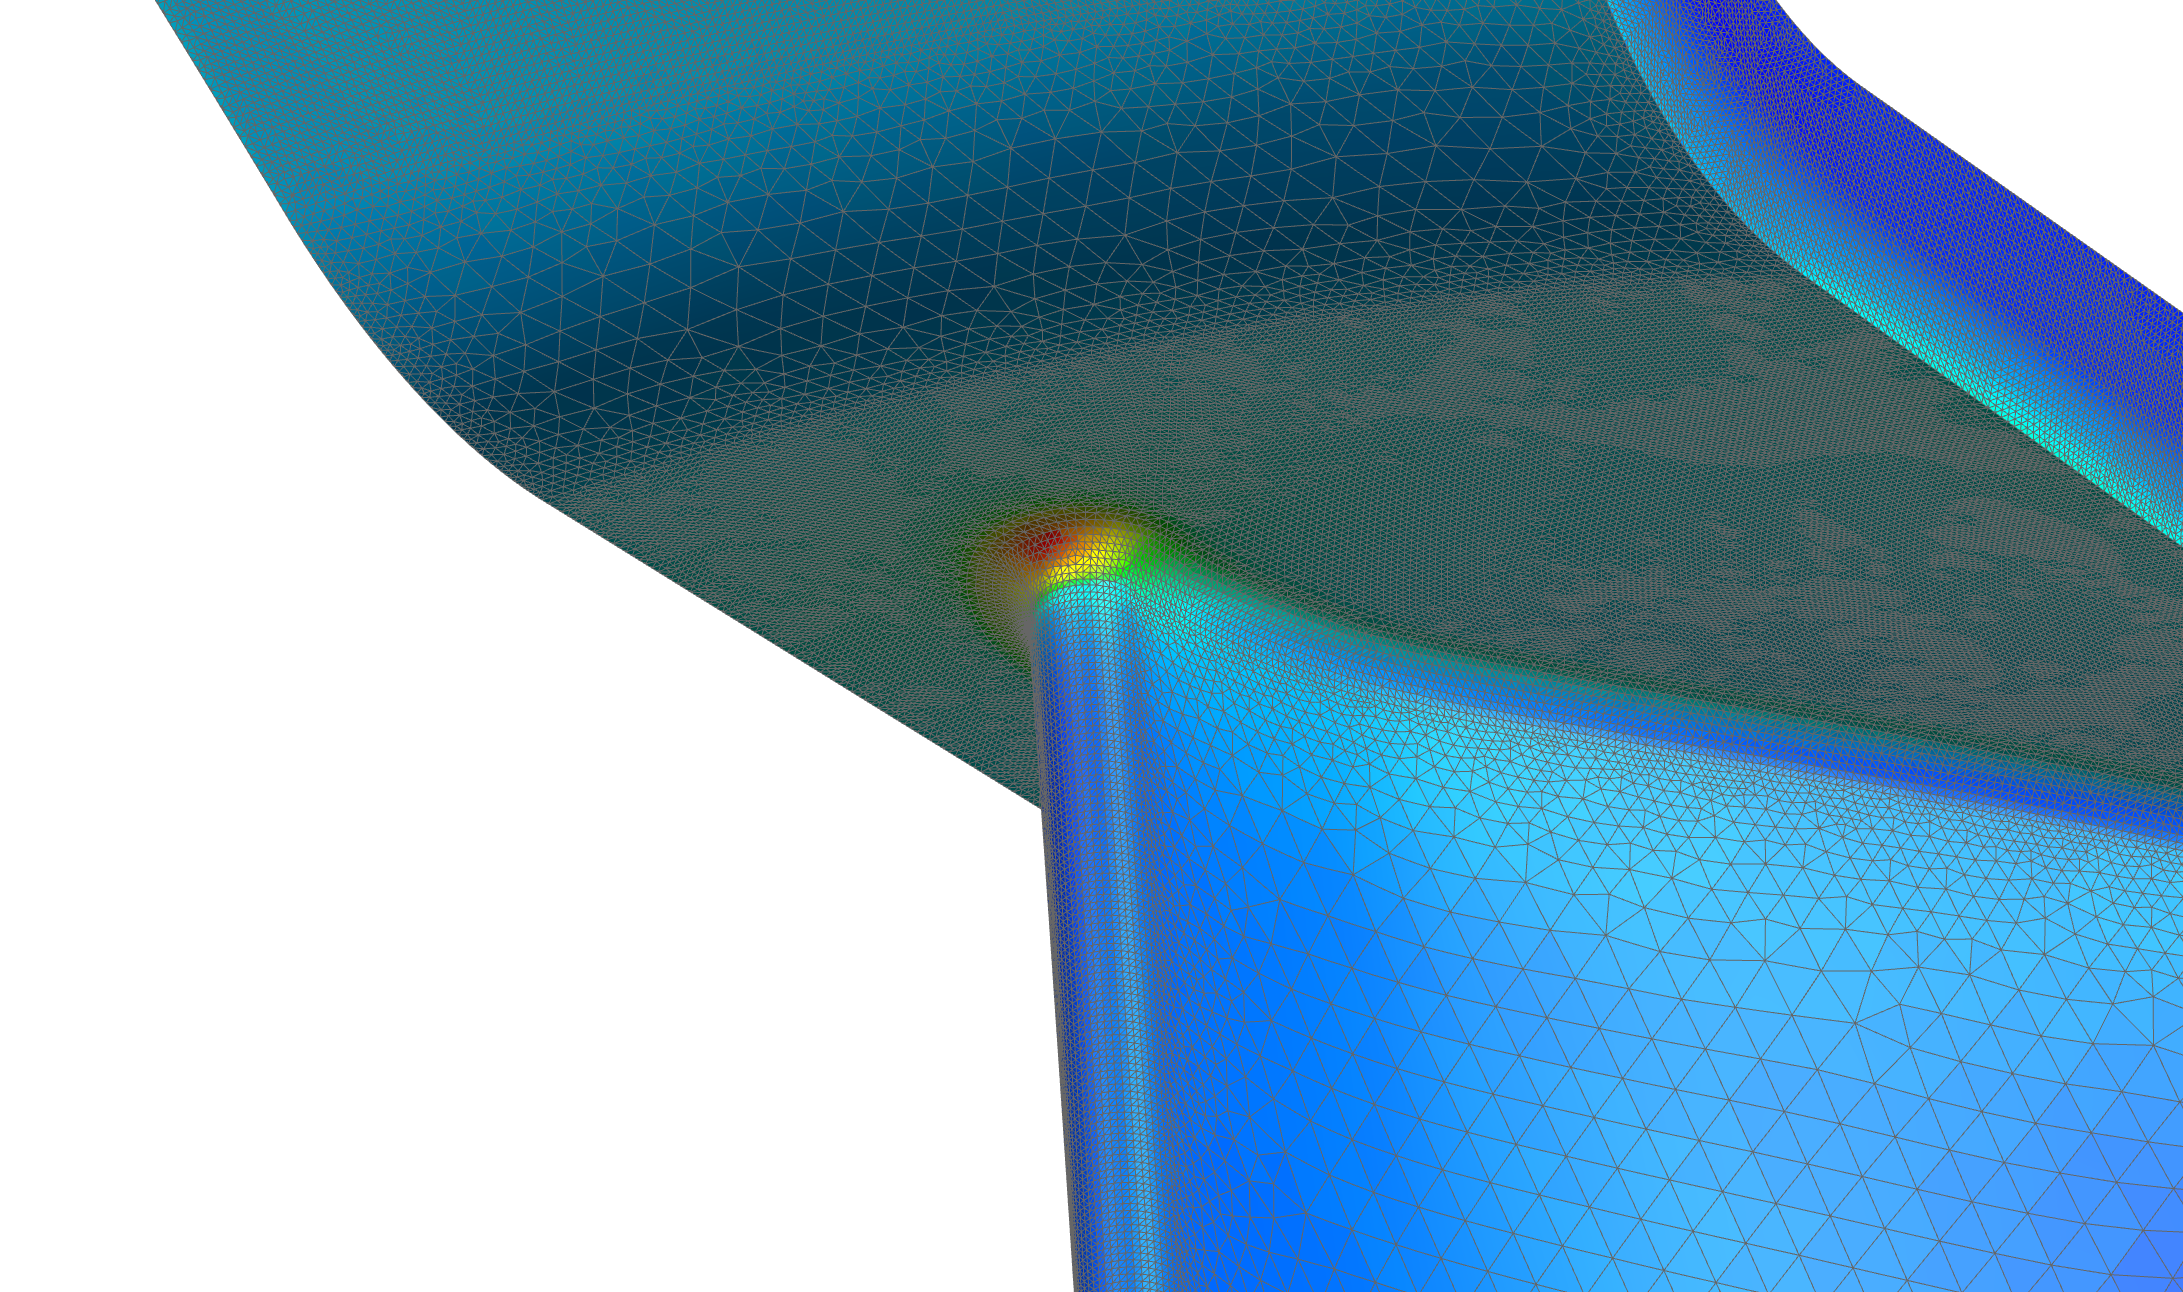
\includegraphics[width=0.8\linewidth]{Figures/stator_shutdown.png}
 	\caption{Maximum stress during shut-down condition}
    \label{stator1}
 \end{figure}

The reason that the stator will crack at this location first is related to the stress due to the temperature difference between the blade and the upper part of the stator. During shut-down conditions, there is a 500 [\textdegree C[] difference between these two. This will cause the upper part of the stator to expand more than the blade below. The upper part of the stator tries to expand in all directions, so it pulls on the upper part of the blade. The blade, especially at the leading edge, does not have a lot of material to prevent this expansion; this causes much tension at the top part of the blade. 

The highest stress found during the shut-down condition is near 2616 [MPa] when considering nodal stress, 2380 [MPa] when considering elemental stress. This value is valid due to the fact that it has a convergence percentage of 9 \%. This percentage is below the 10 \% convergence which is aimed for. See Appendix \ref{AppendixD} for  information about convergence.

\subsection{Operating conditions}
The origin of cracking for operating conditions, where the middle part of the stator is 750 [\textdegree C], is also determined using FEM-analysis. After completing a thermo-elastic analysis and checking for the highest principle stress, the cracking point is found to be at the edge between the bottom backside of the stator and the thin tail part of the stator, as can be seen in Figure \ref{stator2}. 

\begin{figure} [H]
 	\centering
 	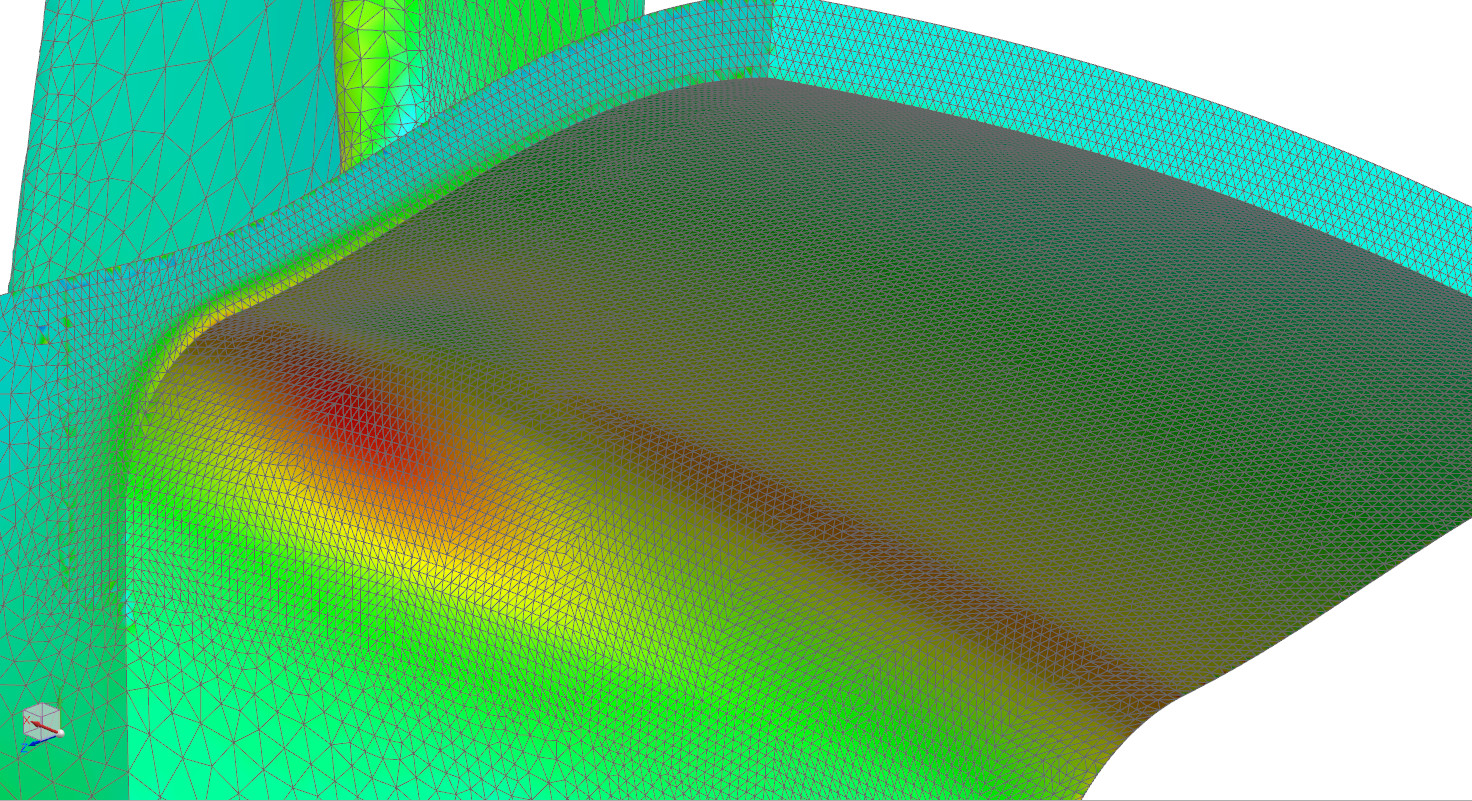
\includegraphics[width=0.8\linewidth]{Figures/0_075OriginalOperating.PNG}
 	\caption{Stator with stresses during operating conditions}
    \label{stator2}
 \end{figure}

The stator will crack at that point due to the resulting stress of the temperature differences between the lower part and the middle part of the stator. In this situation, the difference is about 400 [\textdegree C], which is the highest temperature difference in the stator. The lower temperature of the bottom part of the stator will cause it to expand more than the higher middle part of the stator; this will cause a tension between the bottom part and lower middle part of the stator. This tension is the highest around the edge between the bottom backside and the thin tail part of the stator because the thin tail part of the stator has much less material to distribute the tension to.

The highest stress found during the working condition is around 2217 [MPa] nodal and 2032 [MPa] elemental stress. This value is valid due to the fact that it has a convergence percentage of 8.3 \%, which is below the 10 \% convergence aimed for.
\newpage
\section{Stator redesign: Wave}
\label{Chap:stator_redesign}
Using the problem analysis in Chapter \ref{Chap:stator_analysis}, some changes have been made to reduce the stresses of the stator during operational and shut-down conditions. The changes are made based on the RPCs (see Appendix \ref{AppendixF}), considering all requirements, constraints and preferences. This chapter will address which changes are made, why they are made, and what effect the change has for the stresses. Then, the results for both conditions will be given. In Figure \ref{fig:final_stator}, the re-designed stator is shown, where the numbers indicate an area where a change was made to the original stator.
\begin{figure}[H]
\centering
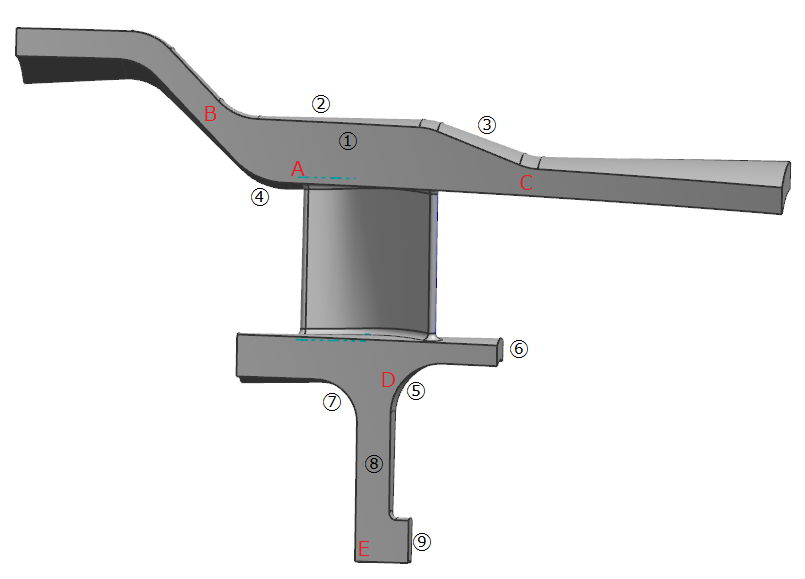
\includegraphics[width=0.8\textwidth]{Figures/final_stator.png}
\caption{The re-designed stator with the indicated changes (1,2,..,9) and high stress points (A,B,..,E).}
\label{fig:final_stator}
\end{figure}
A design is made which is called the 'wave'. Due to its shape, the temperature gradient is lower around the blade-stator transition, where originally the highest stress occurred during the shut-down condition \cite{temperaturepressure}. The high stress points during the operating conditions are related to the shape of the bottom. The bigger edges and thicker planes are successful in lowering the stress. 

\subsection{Description of changes}
\begin{enumerate}
\item The wave itself can be adapted in three dimensions: the length (1), height (2) and angle (3). As said, the temperature gradient will be lower in the blade-stator transition (A), but the wave creates higher stress in the diagonal part (B) and beneath the angle (C). Due to the deformation around these points, the stresses will increase. 
\item The curve in point (4) is moved towards the blade-stator transition; this is done in order to create a larger angle in the diagonal part.
\item To reduce the stress in the lower part of the stator (in operating condition), the temperature gradient must be lowered in and around the edge blend. This is done by increasing the radius of the edge blend in point (5).
\item The beam connected to the edge blend (6) is made a little thicker, which will lower the very high temperature gradient in this part. By lowering the gradient, the deformation will be less, and, therefore, the stress in the edge blend will be lowered.
\item The vertical tail part (8) has been moved towards the center below the blade; this is done in order to create a larger possible radius for the edge blend.
\item The radius of the edge blend in point (7) increased as well; this is again done to lower the temperature gradient at this point.
\item The last change is made to the lid (9), which is reversed in comparison to the original stator. This change is based on the air flow that the stator will endure. There will be less pressure on the vertical tail part, because the air will not get stuck in the 'bowl' created by the lid, tail and surface beneath the blade, since the air will flow from the left looking at Figure \ref{fig:final_stator}.
\end{enumerate}
A FEM analysis will be applied to the redesign of the stator; the results can be seen in Chapter \ref{Results}. An alternative design that is investigated but eliminated can be found in Appendix \ref{AppendixA3}.

\subsection{Compatibility \& Functionality}
As mentioned in the RPCs (Appendix \ref{AppendixF}), the stator is constrained to remain functional and compatible with the stator. Therefore, the 'wave' design should comply with these constraints; otherwise, it can not be used for a jet engine. The compatibility requires that the total jet engine can be assembled correctly with the newly designed stator. Figure \ref{fig:compatible} shows the position of the stator in the jet engine.
\begin{figure}[H]
\centering
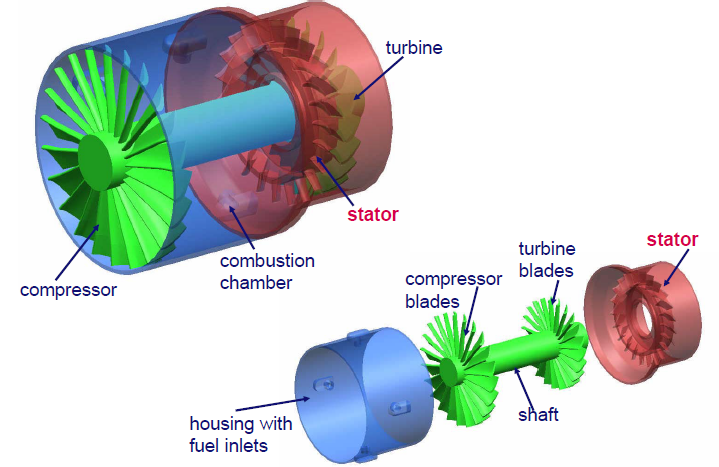
\includegraphics[width=0.6\textwidth]{Figures/compatible.png}
\caption{The compatibility of the stator in the total jet engine and in an exploded view \cite{COC}}
\label{fig:compatible}
\end{figure}
The 'wave' design stator can be compared with the stator in the figure shown above. As you can see, there is not much of a change in the contact area between the stator and the compressor shaft or housing. Therefore, it can be concluded that the 'wave' design remains compatible.

The functionality constraint states that the stator should still be able to convert the increased rotational kinetic energy, caused by the blade, into static pressure. According to the 4GC00 COC, which included Figure \ref{orange outline}, it is not allowed to make adjustments to the blade \cite{COC}. In addition, the surface around the blade, which is in contact with the inflowing air, is barely changed. This means that the functionality will not change with the original stator. The 'wave' design agrees with both the compatibility and functionality constraint.  
\newpage
\section{Analysis of Results}
\label{Results}
\subsection{Results}
According to the converging path of the elemental and nodal stresses for decreasing mesh sizes, the results of the FEM simulation of the final stator have been validated. Local mesh refinements have been applied to the high stress regions to converge even more. Table \ref{tab:final_stresses} shows the maximum stresses for the stator during both the operational and shutdown condition. In this table, the top part of the stator is above the blade while the bottom part is beneath the blade.
\begin{table}[H]
\centering
\caption{Final max principal stress values in the critical areas.}
\label{tab:final_stresses}
\begin{tabular}{|l|l|l|l|}
\hline
\textbf{Condition} & \textbf{Highest stress} [MPa] & \textbf{Convergence [\%]} & \textbf{Location} \\ \hline
Operational        & 810             & 1.1			& Bottom             \\ \hline
Shut-down          & 1505            & 2.5			& Top                \\ \hline
\end{tabular}
\end{table}
\subsection{Validation of the results}
The results for the stator during the shut-down condition show that the stress in the top part exceeds the yield stress, so in reality, the stator will fail in the top part of the stator. The stresses in point (A), (B), and (C) of Figure \ref{fig:final_stator} are all related to the design of the wave and considered when determining the length, height and angle of the wave. The stresses in these points are more or less the same and equal to a value around 1500 [MPa], the high stresses can be seen in Figure \ref{fig:highstressshutdownl}, \ref{fig:highstressshutdown2} and \ref{fig:highstressshutdown3}. The high stresses in shutdown condition exceed the yield stress of the material; therefore in reality, the stator will fail in these points.\\
In operating conditions, the highest stress is equal to 810 [MPa] in the large edge blend below the blade and can be seen in Figure \ref{fig:highstressoperational1}. The convergence percentage that is used to validate the stator is 10$\%$, as can be seen in Appendix \ref{AppendixD}. As can be seen in Table \ref{tab:final_stresses}, the convergence percentage is reached for both conditions. 

Other high stresses occur at the rectangular edge (point (E) in Figure \ref{fig:final_stator}) and the blade edge. The stress on the rectangular edge, which can be seen in Figure \ref{fig:highstressoperational3}, is due to a singularity on this edge and the stress in this singularity can be neglected. Once an edge blend is added to this edge the stress around this edge blend easily becomes lower than the 810 [MPa] in the other high stress point. However, the edge blend will not be applied to the re-design otherwise the compatibility becomes questionable due to a smaller contact surface. The high stress in the blade, which can be seen in Figure \ref{fig:highstressoperational2}, lies within the 1.5 [mm] area of the negligible stresses due to the singularities. However, the stress above the 1.5 [mm] is just a little lower than the highest stress in the edge blend.

\subsection{Deformation}
In the two different circumstances in which the stator operates, a deformation in the material is present. The original stator deforms with a maximum of 0.5 [mm] during the operational conditions. The amount of deformation of the new design is not very different from the original stator design. The main goal of the design is to avoid cracking of the stator, which is caused by the high stress points and not by the deformation amount. Added to that, the correlation between deformation and functionality of the stator remains unknown, but since the deformation is similar to the original, there should be no functionality problem. Therefore, the only major influence on the functionality of the stator is  the amount of stress in the stator compared to the yield stress of the stator.



 
















\newpage
\section{Manufacturing}
\label{manufacturing}
The final stator has to be created from the cast part; the casting model is the blue outline in Figure \ref{fig:finishedmanu}. In order for the stator to reach its final redesign, a manufacturing plan must be created. All the process steps have numbers, outlined below. The premachine steps focus mainly on removing material and will complete multiple passes until an adequate amount of material is removed. Finishing, on the other hand, will only use one pass to smooth the edges of the part. The whole part will be made using a lathe \cite{lathe}. The steps and corresponding tools can be found in Table \ref{manutable} in Appendix \ref{appendixmanufacturing}. The manufacturing plan is as follows:
\begin{enumerate}
\item The first step is creating the hole in the middle of the stator. This hole will have a diameter of 30 [mm] and will be drilled through depth of the whole part.
\item Next, the top part of the stator, labeled A in Figure \ref{fig:finishedmanu}, will be machined. In this step, the level surfaces will be turned as well as pieces of the edges. In Figure \ref{fig:premachining}, the part is visualized after this premachining stage. The level surfaces of the stator are turned, but the edge is only in a preliminary stage; this is visualized using a stair step pattern along the edge.
\item After the premachining is completed, the edges in B will be finished. The edges will be smoothed out to change from the stair step pattern seen in Figure \ref{fig:premachining} to the smooth edges seen in Figure \ref{fig:finishedmanu}.
\item Next, the stator is rotated and a similar process will occur as did in Step 2. The areas labeled B in Figure \ref{fig:finishedmanu} will now be turned. Most of the material will be removed at the upper curve and the lower curve, while the flat surfaces at the lower part of B will be finished. Again, the resulting stair step pattern is visible in Figure \ref{fig:premachining}. For this turning step, the tool used will be different because we are now tooling internally rather than externally.
\item Now the edges in B will be smoothed and finished. This will result in edges like those seen in Figure \ref{fig:finishedmanu}.
\item The stator will be turned once more to machine area C. Again, the flat edges will be turned and the curve at C will be preliminarily turned.
\item Lastly, the finishing will occur for the edge in area C. 
\end{enumerate}

\begin{figure}[H]
\centering
\begin{minipage}{.5\textwidth}
  \centering
  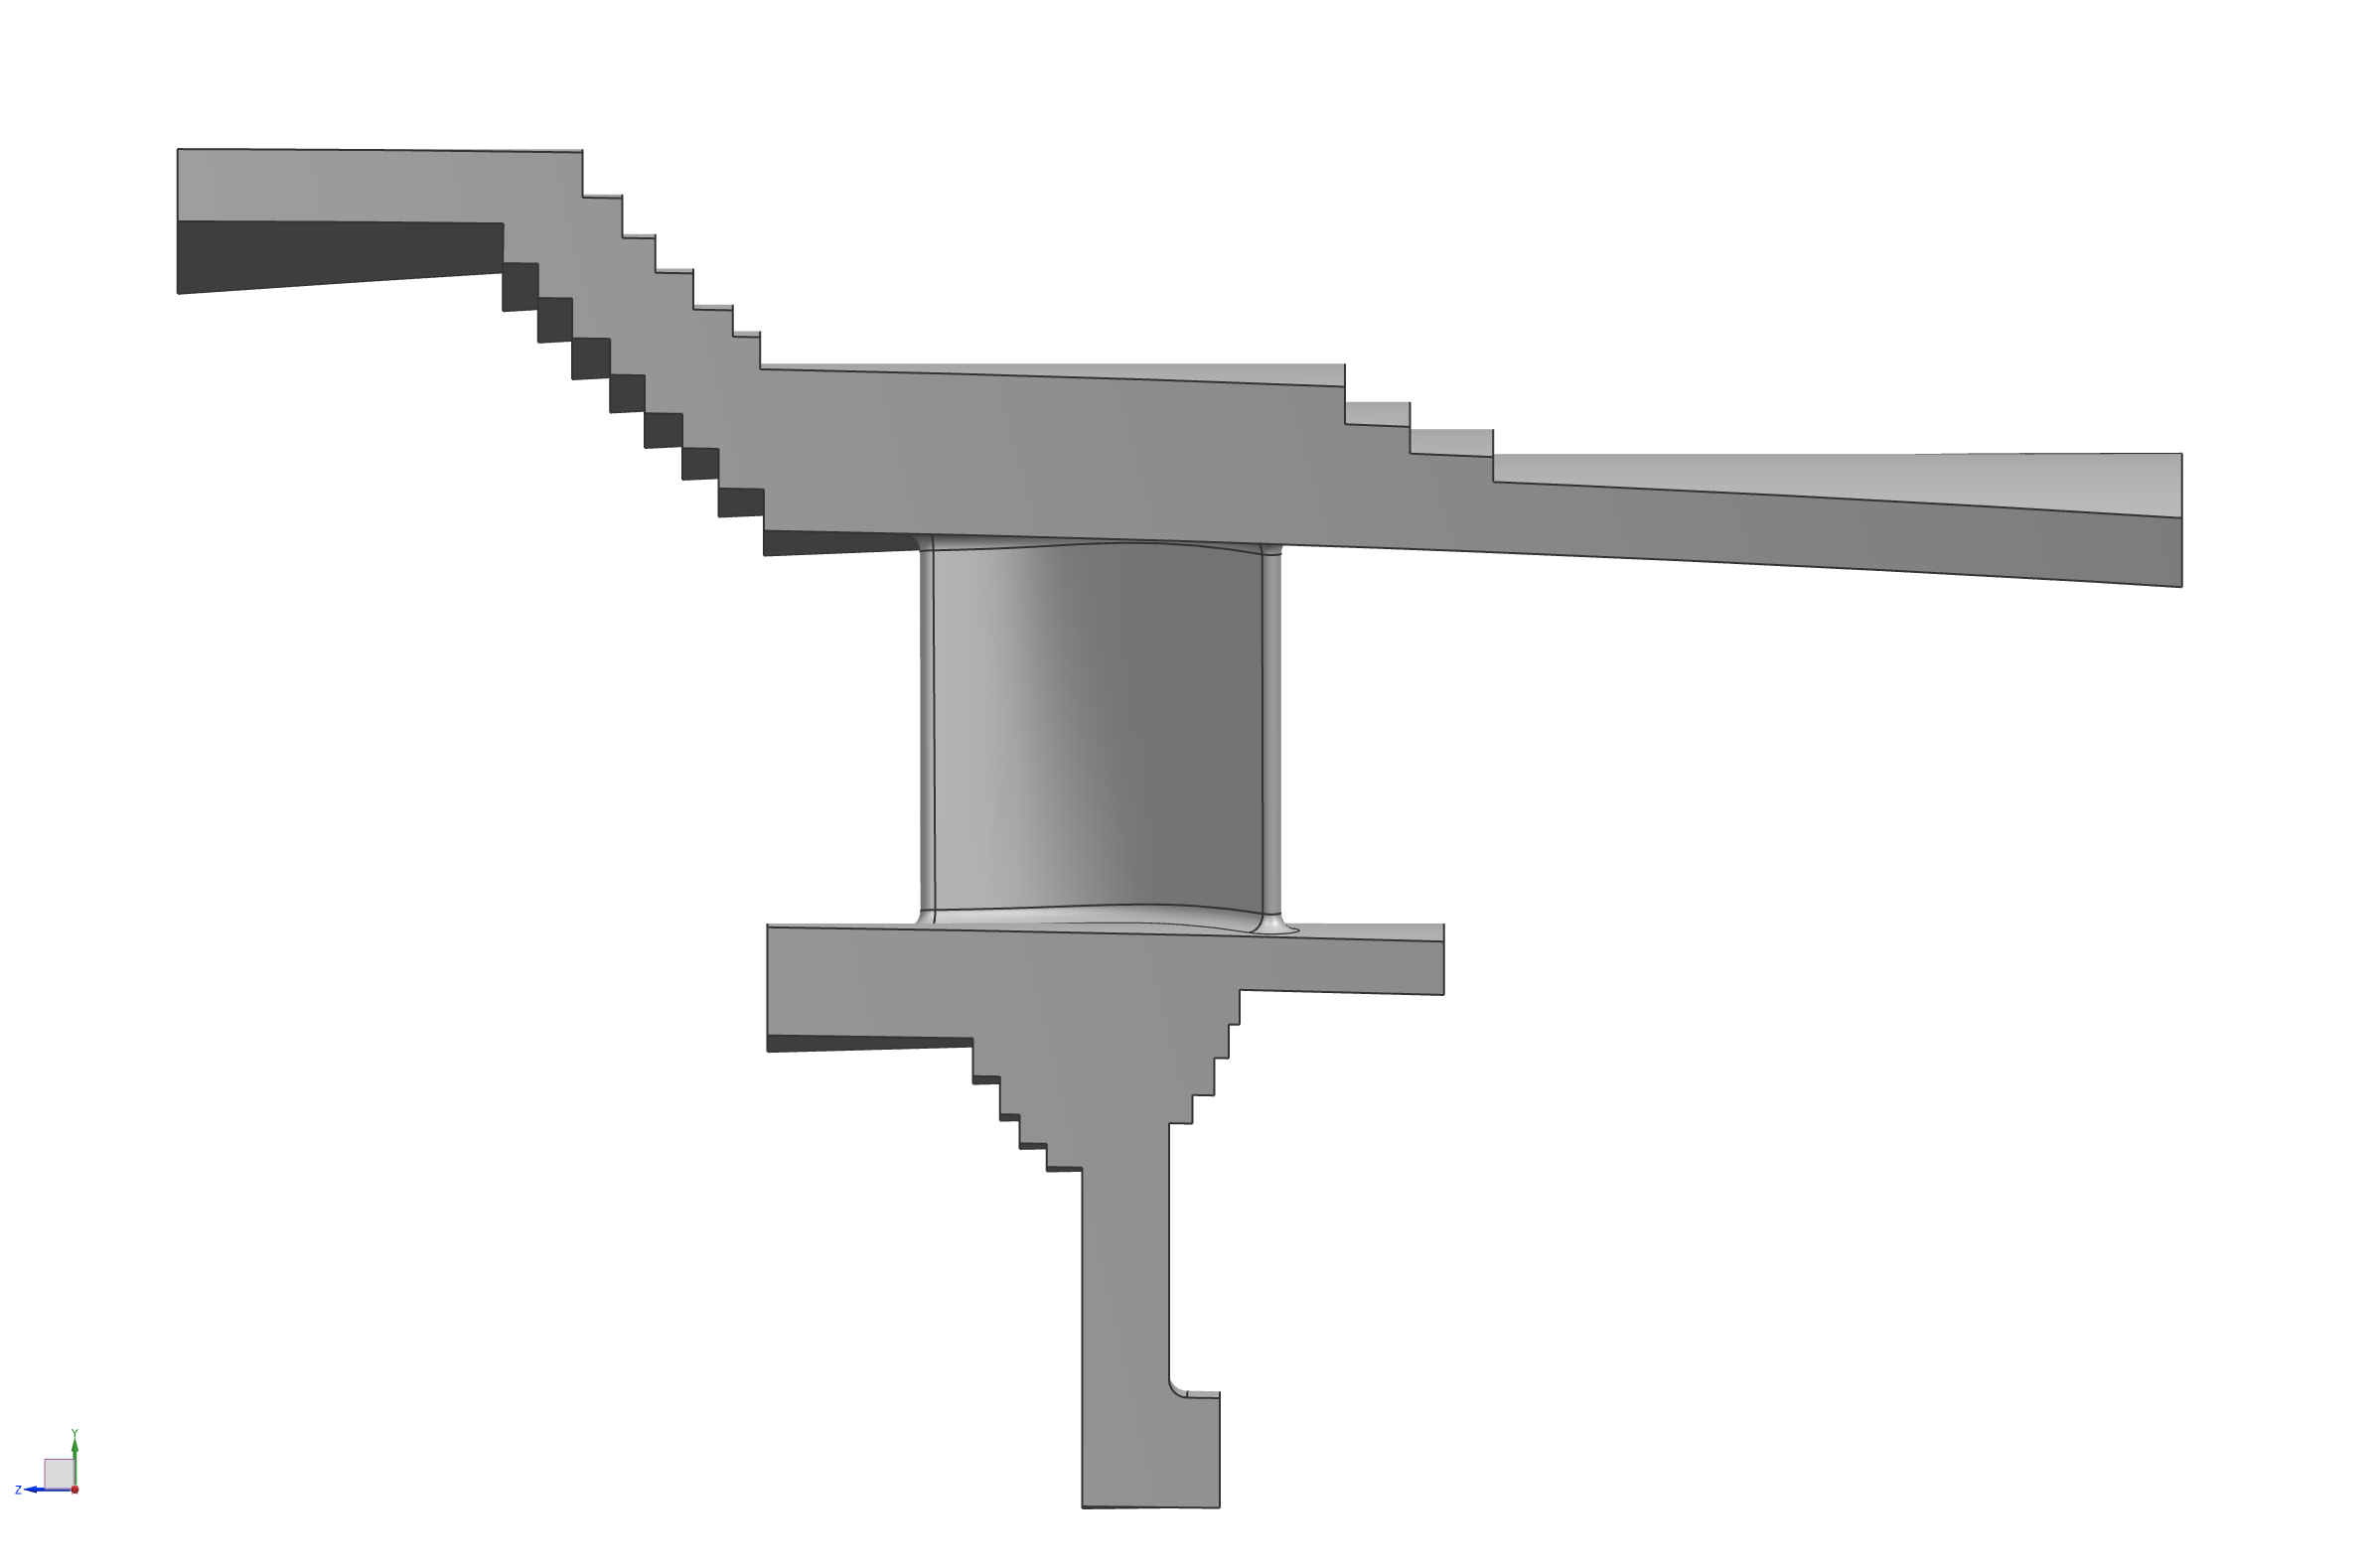
\includegraphics[width=1\linewidth]{Figures/manufacturingpart1.png}
  \captionof{figure}{Premachined Part}
  \label{fig:premachining}
\end{minipage}%
\begin{minipage}{.5\textwidth}
  \centering
  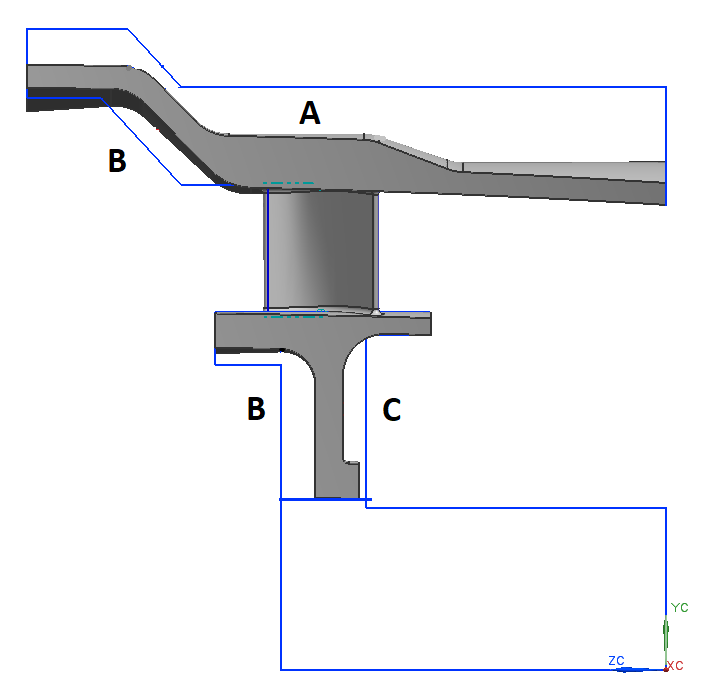
\includegraphics[width=.8\linewidth]{Figures/statormanu2.png}
  \captionof{figure}{Finished Part}
  \label{fig:finishedmanu}
\end{minipage}
\end{figure}

\newpage
\section{Conclusion}
\label{Chap:Conclusion}
The redesigned stator shows great improvements for both the operational and shut-down condition in the high stress areas. The simulated stress in the shut-down condition is lowered from 2616 [MPa] in the original stator to 1505 [MPa] in the redesign; therefore, the durability of the stator is improved. However, the stress in the shut-down condition still exceeds the yield stress of the stator material. This implies that the blade cracking is not prevented and the desired safety factor, as stated in the RPCs, is not reached. In operating conditions the maximum stress is equal to 810 [MPa], this means that the stator will not crack during operating condition. The safety factor is again not reached for this condition. According to the convergence study, the results obtained in the FEM simulations do agree with the convergence percentage; therefore, the accuracy of the FEM analysis is validated. The newly designed stator retains its functionality and is still compatible within the whole jet engine. Furthermore, the manufacturing plan shows that the redesigned stator is manufacturable using common manufacturing techniques. 

\section{Discussion \& Recommendations}
\label{Chap:DiscussionRecommendations}
Multiple assumptions have been made for the analysis of the stator which led to the results and conclusion mentioned above. The most important assumptions will be discussed in this chapter and some recommendations will be given.\\
\begin{itemize}
\item The estimated temperatures of the operation and shut-down condition are a simplified manner to simulate the effect of these conditions on the stator. Furthermore, shutting down the engine is assumed to happen instantly where only one surface changes temperature. 
\item Only the stresses due to the temperature constraints are taken into account; all other sources of stress are neglected. For example, the stress due to the air flow past the stator is disregarded. In addition, the newly created stator is not ensured of a well controlled airflow as no aerodynamic analysis has been done.
\item In the analysis of the cracking points, the high stresses in the blade-stator transition can be neglected due to the singularities in the FEM software; however in reality, the stator will fail in these points. 
\end{itemize}
These assumptions have influences on the final stress result, although some are minor. These assumptions must be taken into account or proven negligible before the stator can be used in a real engine. So is the temperature distribution, used for the analysis, assumed to be much simpler than it can possibly be. Furthermore, the given temperature constraints are probably chosen more extreme than in reality to ensure that the newly designed stator has a small safety margin. Also the influence of the heat flux between the stator and the surrounding air is not taken into account. 

The recommendations follow out of the discussions, these recommendations can be used to better analyze the stator.
\begin{itemize}
\item An aerodynamic analysis should be applied to the stator to determine whether the new curves and edges have any influence on the airflow. Furthermore, the additional stresses caused by the airflow might prove significant enough to no longer be considered negligible. 
\item With the simulations, the number of experiments can be lowered. However, the final design needs to undergo some experiments to assure its applicability to a real jet engine. The stresses that are neglected can cause the stator to fail and this failure can seriously endanger human lives.
\end{itemize}


\newpage
\addcontentsline{toc}{section}{\numberline{}References}
\textit{Later info compleet maken en APA style}

\bibliography{Literature.bib}
\bibliographystyle{unsrt}


\newpage
\newpage
\appendix
\begin{appendices}
\section{Appendix A}
\label{AppendixA}
\subsection{Sample point/lines used in Comsol}

Data is gathered at specific locations in the battery models.
For the 6S1P, the middle point is blabla
\begin{figure} [H]
	\centering
	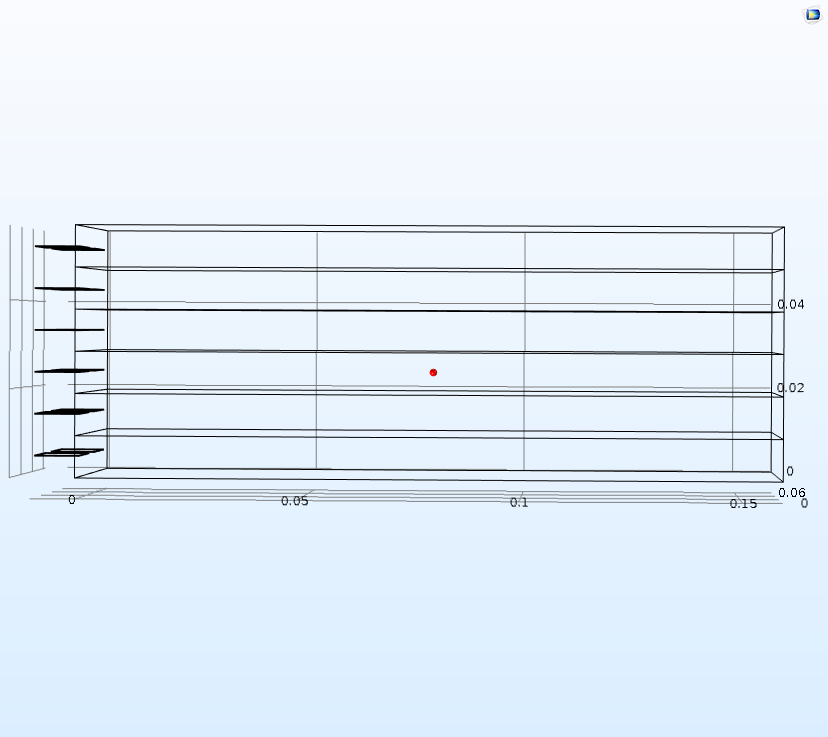
\includegraphics[width=0.5\linewidth]{Figures/6_Point_in_3D.png}
	\caption{Point of measurement in 6S1P simulation.}
   \label{Fig:6_1}
\end{figure}
\begin{figure} [H]
	\centering
	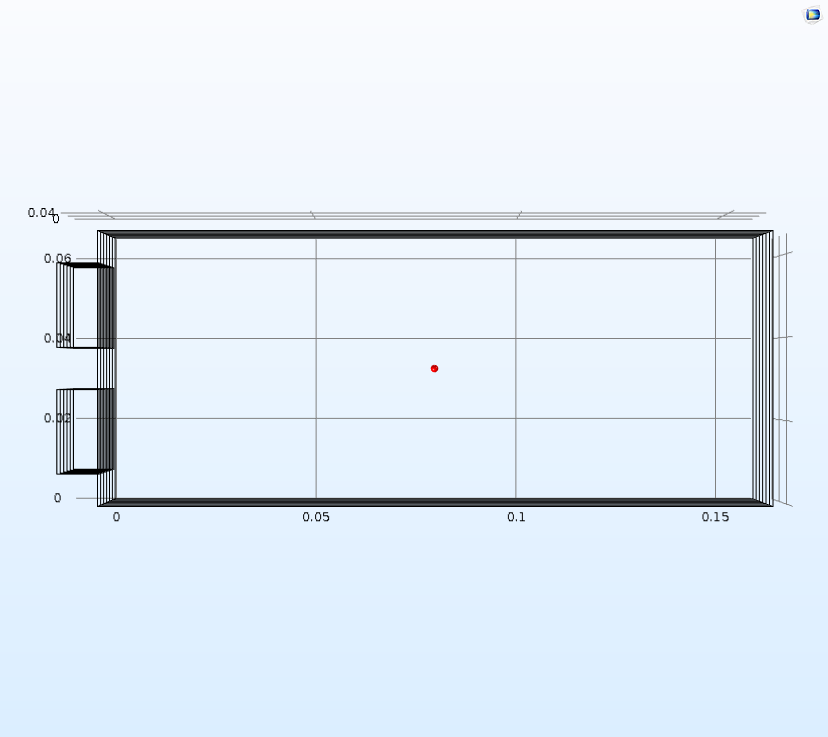
\includegraphics[width=0.5\linewidth]{Figures/6_Point_in_3D_2.png}
	\caption{Point of measurement in 6S1P simulation.}
   \label{Fig:6_2}
\end{figure}

\begin{figure} [H]
	\centering
	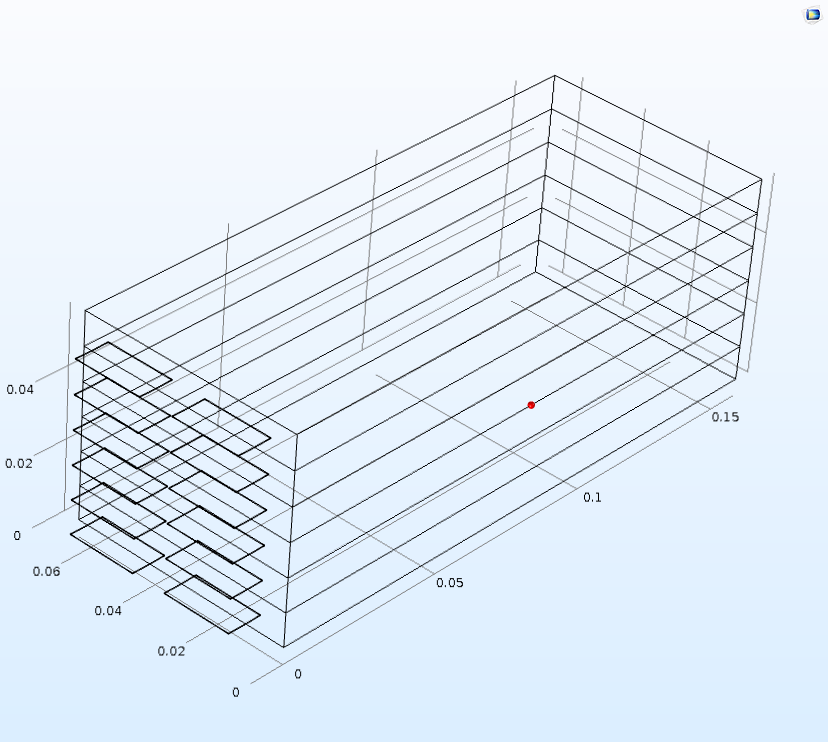
\includegraphics[width=0.5\linewidth]{Figures/6_Point_in_3D_3.png}
	\caption{Point of measurement in 6S1P simulation.}
   \label{Fig:6_3}
\end{figure}

\begin{figure} [H]
	\centering
	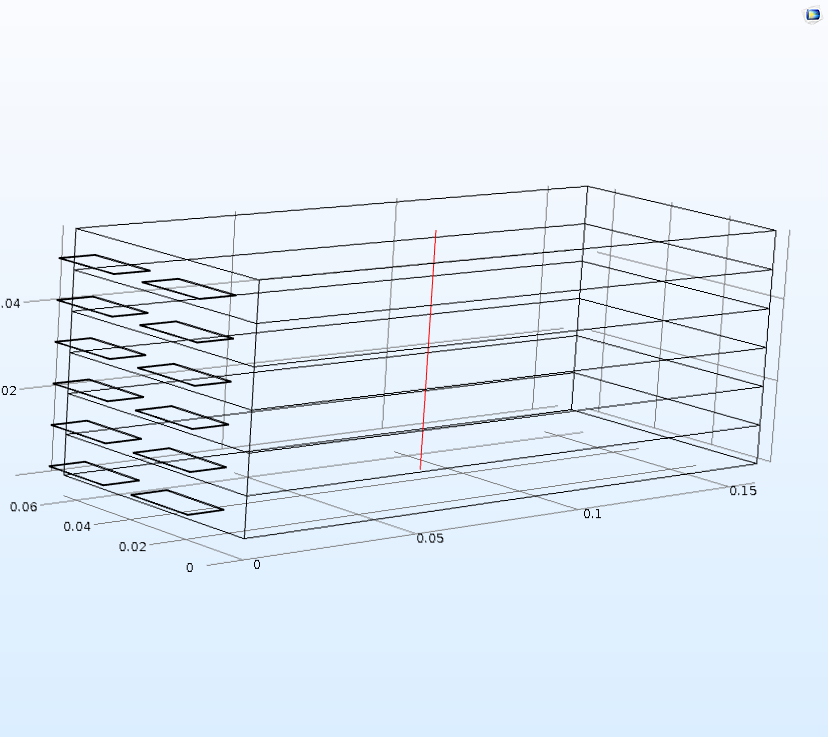
\includegraphics[width=0.5\linewidth]{Figures/LineOutPlane.png}
	\caption{Point of measurement in 6S1P simulation.}
   \label{Fig:6_4}
\end{figure}

\begin{figure} [H]
	\centering
	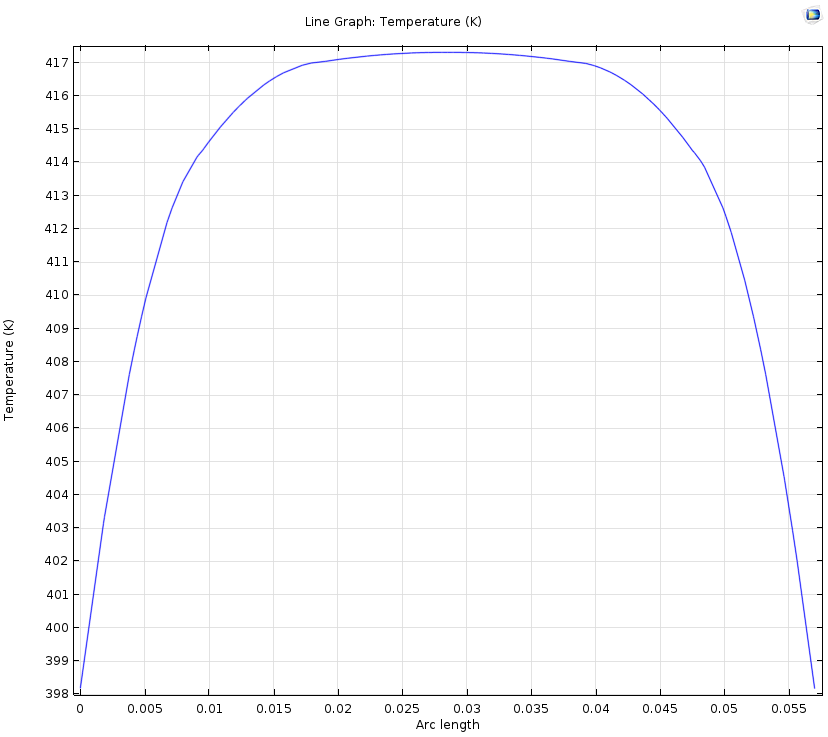
\includegraphics[width=0.5\linewidth]{Figures/300s_10h_180A_2mOhm_OutOfPlaneLast_NoPouch.png}
	\caption{Point of measurement in 6S1P simulation.}
   \label{Fig:6_5}
\end{figure}



\newpage

\end{appendices}

\end{document}
